\documentclass[12pt,a4paper]{article}
\usepackage[margin=22mm]{geometry}
\usepackage{fontspec}
\usepackage{xeCJK}
\usepackage{kotex}
\usepackage{graphicx}
\usepackage[table]{xcolor}
\usepackage{longtable}
\usepackage{booktabs}
\usepackage{array}
\usepackage{ragged2e}
\usepackage{enumitem}
\usepackage{hyperref}
\usepackage{amssymb}
\usepackage{fancyhdr}
\usepackage{titlesec}
\usepackage{setspace}
\setmainfont[Path=C:/Windows/Fonts/, BoldFont=malgunbd.ttf, ItalicFont=malgunsl.ttf]{malgun.ttf}
\setsansfont[Path=C:/Windows/Fonts/, BoldFont=malgunbd.ttf, ItalicFont=malgunsl.ttf]{malgun.ttf}
\setmonofont{Consolas}
\newfontfamily\jpfont[Path=C:/Windows/Fonts/]{NotoSansJP-VF.ttf}
\setCJKmainfont[Path=C:/Windows/Fonts/, BoldFont=malgunbd.ttf, ItalicFont=malgunsl.ttf]{malgun.ttf}
\setCJKsansfont[Path=C:/Windows/Fonts/, BoldFont=malgunbd.ttf, ItalicFont=malgunsl.ttf]{malgun.ttf}
\setCJKmonofont[Path=C:/Windows/Fonts/]{malgun.ttf}
\XeTeXlinebreaklocale "ko"
\hyphenpenalty=10000
\exhyphenpenalty=10000
\binoppenalty=10000
\relpenalty=10000
\emergencystretch=2em
\sloppy
\newcommand{\DocNeedspace}[1]{\par\ifdim\dimexpr\pagegoal-\pagetotal\relax<#1\newpage\fi}
\hypersetup{colorlinks=true, linkcolor=black, urlcolor=blue}
\definecolor{DarkCharcoal}{HTML}{222222}
\definecolor{MainOrange}{HTML}{F26518}
\definecolor{MutedBrown}{HTML}{D44A14}
\definecolor{SoftBeige}{HTML}{FFF3E7}
\definecolor{CardPeach}{HTML}{FCE7DB}
\definecolor{SubTextGray}{HTML}{666666}
\color{DarkCharcoal}
\colorlet{LovvGreen}{MutedBrown}
\colorlet{LovvGreenDark}{DarkCharcoal}
\colorlet{LovvGold}{MainOrange}
\colorlet{LovvPaper}{SoftBeige}
\renewcommand{\arraystretch}{1.35}
\setlength{\tabcolsep}{2pt}
\setlength{\LTpre}{6pt}
\setlength{\LTpost}{10pt}
\setlength{\LTleft}{\fill}
\setlength{\LTright}{\fill}
\setlist[itemize]{leftmargin=*, itemsep=2pt, topsep=2pt}
\setstretch{1.08}
\setlength{\headheight}{30pt}
\setcounter{tocdepth}{2}
\newcommand{\TocNoChildTight}{\vspace{-0.28em}}
\pagestyle{fancy}
\fancyhf{}
\lhead{\hbox{\makebox[42pt][c]{
\includegraphics[width=38pt,height=13pt,keepaspectratio]{../assets/images/SK-Networks-logo.png}}\hspace{0.7em}\makebox[42pt][c]{
\includegraphics[width=44pt,height=15pt,keepaspectratio]{../assets/images/en-core-logo.png}}\hspace{0.7em}\makebox[42pt][c]{
\includegraphics[width=38pt,height=13pt,keepaspectratio]{../assets/images/playdata-logo.png}}}}
\rhead{\scriptsize v0.2 | Review - V2 기준 작성}
\cfoot{\thepage}
\renewcommand{\headrulewidth}{0.4pt}
\renewcommand{\headrule}{\hbox to\headwidth{\color{LovvGreen}\leaders\hrule height \headrulewidth\hfill}}
\begin{document}
\begin{titlepage}
\thispagestyle{empty}

\noindent \hbox to\textwidth{\makebox[0.28\textwidth][c]{
\includegraphics[width=0.22\textwidth,height=0.82cm,keepaspectratio]{../assets/images/SK-Networks-logo.png}}\hfil \makebox[0.28\textwidth][c]{
\includegraphics[width=0.26\textwidth,height=0.98cm,keepaspectratio]{../assets/images/en-core-logo.png}}\hfil \makebox[0.28\textwidth][c]{
\includegraphics[width=0.22\textwidth,height=0.82cm,keepaspectratio]{../assets/images/playdata-logo.png}}}
\vspace{1em}
\par\noindent\color{LovvGold}\rule{\textwidth}{1.2pt}\color{black}

\centering
\vspace*{0.16\textheight}
{\Huge\bfseries V2 기준 AWS 시스템 아키텍처\par}

\vspace{1.5em}
{\large 로브 서비스 V2 배포·운영 아키텍처\par}

\vfill
{\Large\bfseries 조라에몽의 만능 도구들\par}\vspace{0.8em}
{\Large 로브 기획팀\\[0.8em]{\large 멘토 최민수}\par}
\vspace{2em}
{\large 2026-06-29\par}
\end{titlepage}
\begingroup
\fontsize{11.7pt}{12.5pt}\selectfont
\setlength{\parskip}{0pt}
\tableofcontents
\endgroup
\newpage

\newpage

\DocNeedspace{10\baselineskip}
\section*{1. 요약}
\addcontentsline{toc}{section}{1. 요약}
\addtocontents{toc}{\protect\TocNoChildTight}


\DocNeedspace{3\baselineskip}
이 문서는 Lovv 개발 AWS 환경을 V2 도메인 데이터 기준으로 정리한 시스템 아키텍처 문서다.\newline V2 기준은 \texttt{Tour\allowbreak{}Korea\allowbreak{}Domain\allowbreak{}Data\allowbreak{}V2}와 \texttt{lovv-\allowbreak{}vector-\allowbreak{}dev /\allowbreak{} kr-\allowbreak{}tour-\allowbreak{}domain-\allowbreak{}v2}를 향후 추천/RAG 도메인 데이터의 기준선으로 둔다는 뜻이다.


\DocNeedspace{3\baselineskip}
단, 2026-06-29 조회 기준 \texttt{Tour\allowbreak{}Korea\allowbreak{}Domain\allowbreak{}Data\allowbreak{}V2}는 생성되어 있고 KR pipeline Lambda 환경도 V2 테이블과 V2 vector index를 바라보지만, DynamoDB item count는 \texttt{0}이다.\newline 따라서 V2는 문서와 파이프라인 기준선으로 작성하되, 실제 사용자 응답 경로의 cutover는 V2 적재, 인덱싱, API smoke test가 끝난 뒤 진행해야 한다.\newline 기존 \texttt{Tour\allowbreak{}Korea\allowbreak{}Domain\allowbreak{}Data}와 \texttt{kr-\allowbreak{}tour-\allowbreak{}domain-\allowbreak{}v1}은 cutover 전 fallback/reference로 유지한다.


\DocNeedspace{3\baselineskip}
현재 Lovv 개발 AWS 환경은 \texttt{us-\allowbreak{}east-\allowbreak{}1}을 주 리전으로 사용한다.\newline API Gateway, Lambda, Cognito, RDS, DynamoDB, S3 Vectors, VPC 리소스는 대부분 \texttt{us-\allowbreak{}east-\allowbreak{}1}에 있으며, \texttt{ap-\allowbreak{}northeast-\allowbreak{}2}는 Seoul frontend S3/CloudFront 원본과 AgentCore runtime 보조 버킷 흔적 중심으로 확인된다.


\DocNeedspace{16\baselineskip}
\begin{small}
\setlength{\tabcolsep}{3pt}
\setlength{\extrarowheight}{1pt}
\renewcommand{\arraystretch}{1.42}
\begin{longtable}{@{}>{\RaggedRight\arraybackslash}m{0.216\linewidth}>{\RaggedRight\arraybackslash}m{0.756\linewidth}@{}}
\toprule
\multicolumn{1}{>{\centering\arraybackslash}m{0.216\linewidth}}{\textbf{영역}} & \multicolumn{1}{>{\centering\arraybackslash}m{0.756\linewidth}}{\textbf{V2 기준 구조}} \\
\midrule
\endhead
{\footnotesize Frontend/\allowbreak{}CDN} & S3 정적 웹 자산 + CloudFront frontend 2개, 이미지 전용 CloudFront 1개 \\
{\footnotesize API/\allowbreak{}Application} & API Gateway HTTP API \texttt{lovv-\allowbreak{}dev-\allowbreak{}api} -> Python 3.12 Lambda 기능군 \\
Data Stack & CloudFormation stack \texttt{lovv-\allowbreak{}dev-\allowbreak{}data-\allowbreak{}stack}이 VPC, private RDS, DynamoDB, S3 image bucket, VPC endpoint, NAT instance를 소유 \\
V2 Domain/RAG & \texttt{Tour\allowbreak{}Korea\allowbreak{}Domain\allowbreak{}Data\allowbreak{}V2}, \texttt{kr-\allowbreak{}tour-\allowbreak{}domain-\allowbreak{}v2}, Bedrock AgentCore Runtime, KR pipeline Lambda \\
V1 Fallback & \texttt{Tour\allowbreak{}Korea\allowbreak{}Domain\allowbreak{}Data}, \texttt{kr-\allowbreak{}tour-\allowbreak{}domain-\allowbreak{}v1}은 V2 cutover 전 검증/대체 경로로 유지 \\
\bottomrule
\end{longtable}
\end{small}


\newpage

\DocNeedspace{10\baselineskip}
\section*{2. 전체 구성도}
\addcontentsline{toc}{section}{2. 전체 구성도}
\addtocontents{toc}{\protect\TocNoChildTight}



\begin{center}
\vspace*{0.02\textheight}
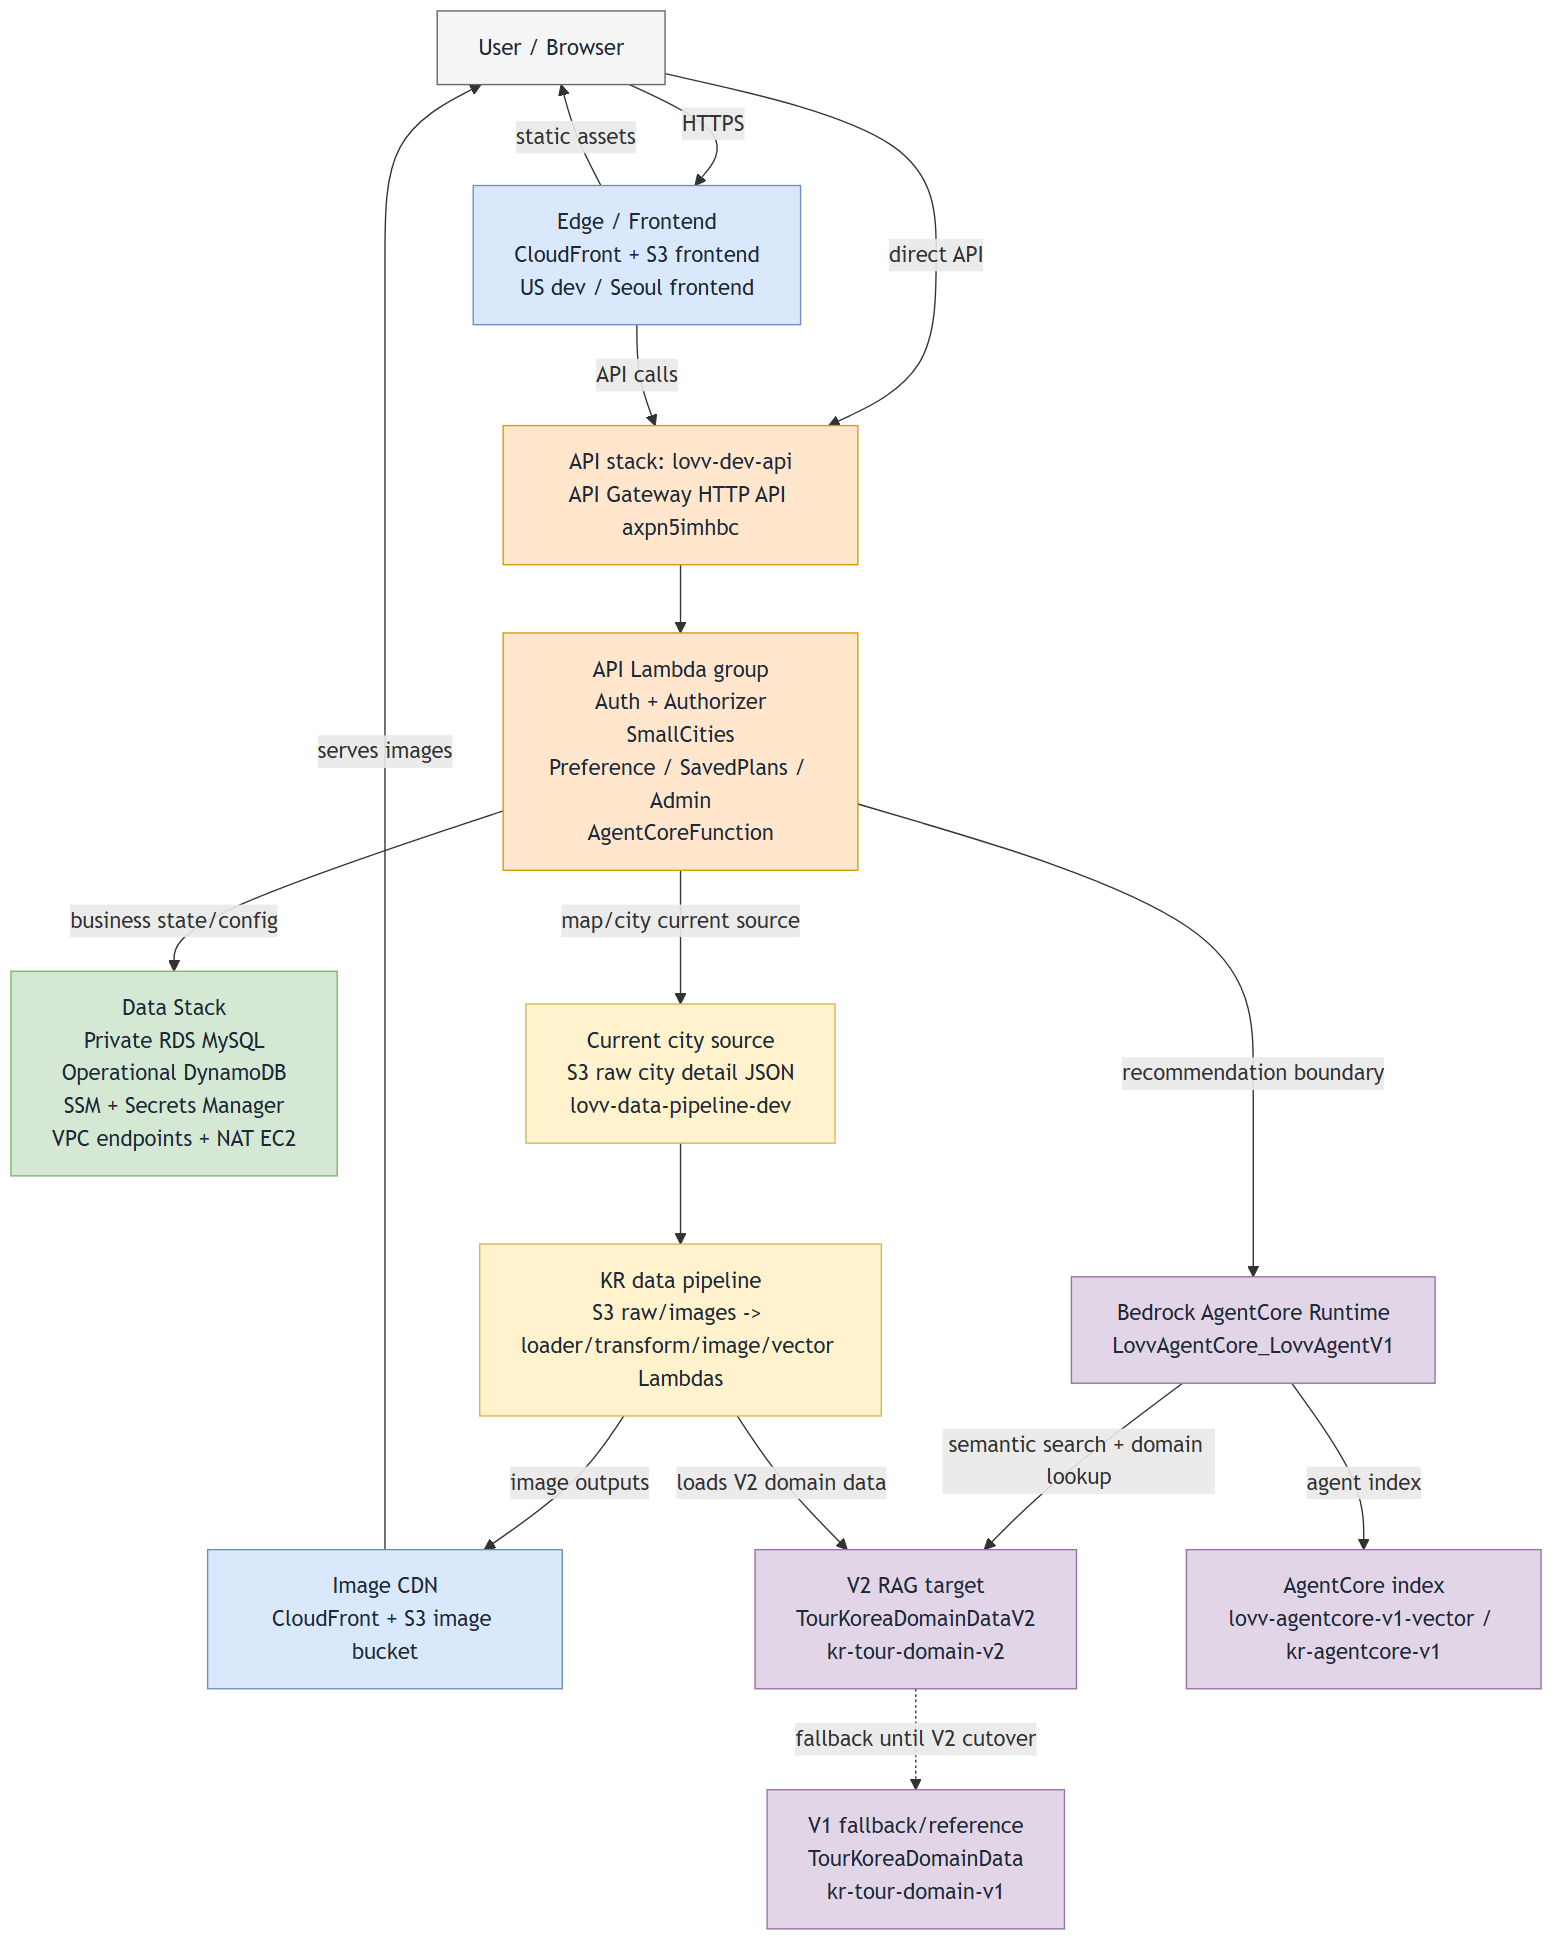
\includegraphics[width=0.84\linewidth,height=0.76\textheight,keepaspectratio]{../docs/11_deployment_ops/supplemental/current_aws_system_architecture.png}
\vspace{0.6em}

{\small V2 기준 시스템 아키텍처: AgentCore Runtime, TourKoreaDomainDataV2, kr-tour-domain-v2, V1 fallback과 현재 SmallCities S3 raw source를 분리해 표시한다.}
\end{center}


\newpage

\DocNeedspace{10\baselineskip}
\section*{3. 현재 확인된 AWS 리소스}
\addcontentsline{toc}{section}{3. 현재 확인된 AWS 리소스}


\DocNeedspace{8\baselineskip}
\subsection*{3.1 리전과 스택}
\addcontentsline{toc}{subsection}{3.1 리전과 스택}


\DocNeedspace{10\baselineskip}
\begin{small}
\setlength{\tabcolsep}{3pt}
\setlength{\extrarowheight}{1pt}
\renewcommand{\arraystretch}{1.42}
\begin{longtable}{@{}>{\RaggedRight\arraybackslash}m{0.345\linewidth}>{\RaggedRight\arraybackslash}m{0.627\linewidth}@{}}
\toprule
\multicolumn{1}{>{\centering\arraybackslash}m{0.345\linewidth}}{\textbf{리전}} & \multicolumn{1}{>{\centering\arraybackslash}m{0.627\linewidth}}{\textbf{확인된 상태}} \\
\midrule
\endhead
\texttt{us-\allowbreak{}east-\allowbreak{}1} & API, Data Stack, AgentCore Runtime, RDS, DynamoDB, Lambda, S3 Vectors의 주 리전 \\
\texttt{ap-\allowbreak{}northeast-\allowbreak{}2} & \texttt{lovv-\allowbreak{}frontend-\allowbreak{}dev-\allowbreak{}seoul-\allowbreak{}925273580929}, \texttt{bedrock-\allowbreak{}agentcore-\allowbreak{}runtime-\allowbreak{}925273580929-\allowbreak{}ap-\allowbreak{}northeast-\allowbreak{}2-\allowbreak{}5u7av7fyw} 버킷 확인. CloudFormation/Lambda/DynamoDB/RDS 활성 목록은 비어 있음 \\
\bottomrule
\end{longtable}
\end{small}


\DocNeedspace{20\baselineskip}
\begin{small}
\setlength{\tabcolsep}{3pt}
\setlength{\extrarowheight}{1pt}
\renewcommand{\arraystretch}{1.42}
\begin{longtable}{@{}>{\RaggedRight\arraybackslash}m{0.418\linewidth}>{\RaggedRight\arraybackslash}m{0.164\linewidth}>{\RaggedRight\arraybackslash}m{0.378\linewidth}@{}}
\toprule
\multicolumn{1}{>{\centering\arraybackslash}m{0.418\linewidth}}{\textbf{Stack}} & \multicolumn{1}{>{\centering\arraybackslash}m{0.164\linewidth}}{\textbf{상태}} & \multicolumn{1}{>{\centering\arraybackslash}m{0.378\linewidth}}{\textbf{역할}} \\
\midrule
\endhead
\texttt{lovv-\allowbreak{}dev-\allowbreak{}api} & \texttt{UPDATE\_\allowbreak{}COMPLETE} & HTTP API, Cognito, API Lambda 기능군. 2026-06-29 업데이트 확인 \\
\texttt{lovv-\allowbreak{}dev-\allowbreak{}data-\allowbreak{}stack} & \texttt{UPDATE\_\allowbreak{}COMPLETE} & VPC, RDS, DynamoDB, S3 image bucket, CloudFront image CDN, VPC endpoint, NAT instance \\
\texttt{Agent\allowbreak{}Core-\allowbreak{}Lovv\allowbreak{}Agent\allowbreak{}Core-\allowbreak{}v1} & \texttt{UPDATE\_\allowbreak{}COMPLETE} & Bedrock AgentCore Runtime \texttt{Lovv\allowbreak{}Agent\allowbreak{}V1} \\
\texttt{Agent\allowbreak{}Core-\allowbreak{}Multiturn\allowbreak{}Playground-\allowbreak{}v1} & \texttt{UPDATE\_\allowbreak{}COMPLETE} & AgentCore 실험/플레이그라운드 계열 \\
\texttt{Agent\allowbreak{}Core-\allowbreak{}myagent-\allowbreak{}default} & \texttt{UPDATE\_\allowbreak{}COMPLETE} & AgentCore 기본 실험 계열 \\
\texttt{CDKToolkit} & \texttt{CREATE\_\allowbreak{}COMPLETE} & CDK bootstrap \\
\texttt{aws-\allowbreak{}sam-\allowbreak{}cli-\allowbreak{}managed-\allowbreak{}default} & \texttt{CREATE\_\allowbreak{}COMPLETE} & SAM CLI managed bucket \\
\bottomrule
\end{longtable}
\end{small}


\DocNeedspace{24\baselineskip}
\subsection*{3.2 Frontend/CDN}
\addcontentsline{toc}{subsection}{3.2 Frontend/CDN}


\DocNeedspace{18\baselineskip}
\begin{small}
\setlength{\tabcolsep}{3pt}
\setlength{\extrarowheight}{1pt}
\renewcommand{\arraystretch}{1.42}
\begin{longtable}{@{}>{\RaggedRight\arraybackslash}m{0.116\linewidth}>{\RaggedRight\arraybackslash}m{0.472\linewidth}>{\RaggedRight\arraybackslash}m{0.371\linewidth}@{}}
\toprule
\multicolumn{1}{>{\centering\arraybackslash}m{0.116\linewidth}}{\textbf{리소스}} & \multicolumn{1}{>{\centering\arraybackslash}m{0.472\linewidth}}{\textbf{값}} & \multicolumn{1}{>{\centering\arraybackslash}m{0.371\linewidth}}{\textbf{역할}} \\
\midrule
\endhead
{\scriptsize Cloud\allowbreak{}Front} & \texttt{d3nuef0zacpyj.\allowbreak{}cloudfront.\allowbreak{}net} & \texttt{lovv-\allowbreak{}frontend-\allowbreak{}dev} 원본의 dev frontend 배포 \\
{\scriptsize Cloud\allowbreak{}Front} & \texttt{dkyiemfaw3g04.\allowbreak{}cloudfront.\allowbreak{}net} & \texttt{lovv-\allowbreak{}frontend-\allowbreak{}dev-\allowbreak{}seoul-\allowbreak{}925273580929} 원본의 Seoul frontend 배포 \\
{\scriptsize Cloud\allowbreak{}Front} & \texttt{det7vj7wxfmim.\allowbreak{}cloudfront.\allowbreak{}net} & \texttt{lovv-\allowbreak{}image-\allowbreak{}dev-\allowbreak{}925273580929} 이미지 버킷 read-only CDN \\
S3 & \texttt{lovv-\allowbreak{}frontend-\allowbreak{}dev} & 정적 프론트엔드 자산, \texttt{us-\allowbreak{}east-\allowbreak{}1} \\
S3 & \texttt{lovv-\allowbreak{}frontend-\allowbreak{}dev-\allowbreak{}seoul-\allowbreak{}925273580929} & 정적 프론트엔드 자산, \texttt{ap-\allowbreak{}northeast-\allowbreak{}2} \\
S3 & \texttt{lovv-\allowbreak{}image-\allowbreak{}dev-\allowbreak{}925273580929} & 이미지 저장 버킷, \texttt{us-\allowbreak{}east-\allowbreak{}1} \\
\bottomrule
\end{longtable}
\end{small}


\DocNeedspace{24\baselineskip}
\subsection*{3.3 API/Application}
\addcontentsline{toc}{subsection}{3.3 API/Application}


\DocNeedspace{16\baselineskip}
\begin{small}
\setlength{\tabcolsep}{3pt}
\setlength{\extrarowheight}{1pt}
\renewcommand{\arraystretch}{1.42}
\begin{longtable}{@{}>{\RaggedRight\arraybackslash}m{0.275\linewidth}>{\RaggedRight\arraybackslash}m{0.697\linewidth}@{}}
\toprule
\multicolumn{1}{>{\centering\arraybackslash}m{0.275\linewidth}}{\textbf{리소스}} & \multicolumn{1}{>{\centering\arraybackslash}m{0.697\linewidth}}{\textbf{값}} \\
\midrule
\endhead
API Gateway & HTTP API \texttt{lovv-\allowbreak{}dev-\allowbreak{}api}, id \texttt{axpn5imhbc} \\
API URL & \texttt{https:\allowbreak{}/\allowbreak{}/\allowbreak{}axpn5imhbc.\allowbreak{}execute-\allowbreak{}api.\allowbreak{}us-\allowbreak{}east-\allowbreak{}1.\allowbreak{}amazonaws.\allowbreak{}com} \\
Cognito Hosted UI & \texttt{https:\allowbreak{}/\allowbreak{}/\allowbreak{}lovv-\allowbreak{}dev-\allowbreak{}auth-\allowbreak{}925273580929.\allowbreak{}auth.\allowbreak{}us-\allowbreak{}east-\allowbreak{}1.\allowbreak{}amazoncognito.\allowbreak{}com} \\
Cognito User Pool & \texttt{lovv-\allowbreak{}dev-\allowbreak{}auth-\allowbreak{}users}, id \texttt{us-\allowbreak{}east-\allowbreak{}1\_\allowbreak{}ynar\allowbreak{}AQBR2} \\
Cognito IdP & Google, Kakao \\
\bottomrule
\end{longtable}
\end{small}


\DocNeedspace{20\baselineskip}
\begin{small}
\setlength{\tabcolsep}{3pt}
\setlength{\extrarowheight}{1pt}
\renewcommand{\arraystretch}{1.42}
\begin{longtable}{@{}>{\RaggedRight\arraybackslash}m{0.472\linewidth}>{\RaggedRight\arraybackslash}m{0.139\linewidth}>{\RaggedRight\arraybackslash}m{0.348\linewidth}@{}}
\toprule
\multicolumn{1}{>{\centering\arraybackslash}m{0.472\linewidth}}{\textbf{Lambda}} & \multicolumn{1}{>{\centering\arraybackslash}m{0.139\linewidth}}{\textbf{런타임}} & \multicolumn{1}{>{\centering\arraybackslash}m{0.348\linewidth}}{\textbf{주요 역할}} \\
\midrule
\endhead
\texttt{lovv-\allowbreak{}dev-\allowbreak{}api-\allowbreak{}Auth\allowbreak{}Function-\allowbreak{}*} & Python 3.12 & Google/Kakao login, Cognito bridge session, logout, profile \\
\texttt{lovv-\allowbreak{}dev-\allowbreak{}api-\allowbreak{}Auth\allowbreak{}Authorizer\allowbreak{}Function-\allowbreak{}*} & Python 3.12 & Custom API authorizer \\
\texttt{lovv-\allowbreak{}dev-\allowbreak{}api-\allowbreak{}Small\allowbreak{}Cities\allowbreak{}Function-\allowbreak{}*} & Python 3.12 & map markers, city list/detail, city places. 현재 S3 raw city detail JSON을 읽는 경로로 확인됨 \\
\texttt{lovv-\allowbreak{}dev-\allowbreak{}api-\allowbreak{}Preference\allowbreak{}Function-\allowbreak{}*} & Python 3.12 & user preferences \\
\texttt{lovv-\allowbreak{}dev-\allowbreak{}api-\allowbreak{}Saved\allowbreak{}Plans\allowbreak{}Function-\allowbreak{}*} & Python 3.12 & saved itineraries, public itinerary, reactions, share \\
\texttt{lovv-\allowbreak{}dev-\allowbreak{}api-\allowbreak{}Admin\allowbreak{}Function-\allowbreak{}*} & Python 3.12 & admin data proposals, notices, monthly destinations, metrics, policies \\
\texttt{lovv-\allowbreak{}dev-\allowbreak{}api-\allowbreak{}Agent\allowbreak{}Core\allowbreak{}Function-\allowbreak{}*} & Python 3.12 & \texttt{POST /\allowbreak{}api/\allowbreak{}v1/\allowbreak{}recommendations}, Bedrock AgentCore Runtime 호출 경계 \\
\bottomrule
\end{longtable}
\end{small}


\DocNeedspace{24\baselineskip}
\subsection*{3.4 Data Stack and Network}
\addcontentsline{toc}{subsection}{3.4 Data Stack and Network}


\DocNeedspace{20\baselineskip}
\begin{small}
\setlength{\tabcolsep}{3pt}
\setlength{\extrarowheight}{1pt}
\renewcommand{\arraystretch}{1.42}
\begin{longtable}{@{}>{\RaggedRight\arraybackslash}m{0.142\linewidth}>{\RaggedRight\arraybackslash}m{0.420\linewidth}>{\RaggedRight\arraybackslash}m{0.397\linewidth}@{}}
\toprule
\multicolumn{1}{>{\centering\arraybackslash}m{0.142\linewidth}}{\textbf{리소스}} & \multicolumn{1}{>{\centering\arraybackslash}m{0.420\linewidth}}{\textbf{값}} & \multicolumn{1}{>{\centering\arraybackslash}m{0.397\linewidth}}{\textbf{상태/의미}} \\
\midrule
\endhead
VPC & \texttt{vpc-\allowbreak{}0ccb7e4be7b11b9fb} & 개발용 VPC \\
Private subnets & \texttt{subnet-\allowbreak{}0e04f80cfb58e0f35}, \texttt{subnet-\allowbreak{}0b3d1d99edd282504} & RDS/VPC endpoint 영역 \\
Public subnet & \texttt{subnet-\allowbreak{}0db1616e7e5db8baf} & NAT instance 영역 \\
NAT instance & \texttt{i-\allowbreak{}0c6dad9690abd0101}, \texttt{t4g.\allowbreak{}nano}, running & private subnet outbound/운영 접근 보조 \\
RDS & \texttt{lovv-\allowbreak{}dev-\allowbreak{}mysql}, MySQL 8.0.45, \texttt{db.\allowbreak{}t4g.\allowbreak{}micro}, DB \texttt{lovvdev} & \texttt{Publicly\allowbreak{}Accessible=false}, StorageEncrypted=true, DeletionProtection=true \\
VPC endpoints & S3 Gateway, DynamoDB Gateway, SSM Interface, Secrets Manager Interface & private subnet AWS service 접근 \\
RDS secret & Secrets Manager ARN이 SSM에 등록됨 & 실제 secret 값은 문서화 금지 \\
\bottomrule
\end{longtable}
\end{small}


\DocNeedspace{24\baselineskip}
\subsection*{3.5 V2 Domain Data}
\addcontentsline{toc}{subsection}{3.5 V2 Domain Data}


\DocNeedspace{18\baselineskip}
\begin{small}
\setlength{\tabcolsep}{3pt}
\setlength{\extrarowheight}{1pt}
\renewcommand{\arraystretch}{1.42}
\begin{longtable}{@{}>{\RaggedRight\arraybackslash}m{0.473\linewidth}>{\RaggedRight\arraybackslash}m{0.499\linewidth}@{}}
\toprule
\multicolumn{1}{>{\centering\arraybackslash}m{0.473\linewidth}}{\textbf{리소스}} & \multicolumn{1}{>{\centering\arraybackslash}m{0.499\linewidth}}{\textbf{상태/용도}} \\
\midrule
\endhead
\texttt{Tour\allowbreak{}Korea\allowbreak{}Domain\allowbreak{}Data\allowbreak{}V2} & ACTIVE, V2 도메인 데이터 cutover target. 2026-06-29 조회 기준 item count \texttt{0} \\
V2 GSI & \texttt{City\allowbreak{}Domain\allowbreak{}Index}, \texttt{Festival\allowbreak{}Month\allowbreak{}Index}, \texttt{Province\allowbreak{}Domain\allowbreak{}Index}, \texttt{Entity\allowbreak{}Type\allowbreak{}Domain\allowbreak{}Index} \\
\texttt{lovv-\allowbreak{}vector-\allowbreak{}dev /\allowbreak{} kr-\allowbreak{}tour-\allowbreak{}domain-\allowbreak{}v2} & V2 KR 도메인 추천 검색 인덱스. 2026-06-29 생성 확인 \\
\texttt{Tour\allowbreak{}Korea\allowbreak{}Domain\allowbreak{}Data} & ACTIVE, 8,022 items. V2 cutover 전 fallback/reference \\
\texttt{lovv-\allowbreak{}vector-\allowbreak{}dev /\allowbreak{} kr-\allowbreak{}tour-\allowbreak{}domain-\allowbreak{}v1} & V1 KR 도메인 검색 인덱스. V2 cutover 전 fallback/reference \\
\texttt{lovv-\allowbreak{}agentcore-\allowbreak{}v1-\allowbreak{}vector /\allowbreak{} kr-\allowbreak{}agentcore-\allowbreak{}v1} & AgentCore V1 검색 인덱스. 도메인 V2 전환과 별도로 유지 \\
\bottomrule
\end{longtable}
\end{small}


\DocNeedspace{24\baselineskip}
\subsection*{3.6 Operational DynamoDB Tables}
\addcontentsline{toc}{subsection}{3.6 Operational DynamoDB Tables}


\DocNeedspace{24\baselineskip}
\begin{small}
\setlength{\tabcolsep}{3pt}
\setlength{\extrarowheight}{1pt}
\renewcommand{\arraystretch}{1.42}
\begin{longtable}{@{}>{\RaggedRight\arraybackslash}m{0.458\linewidth}>{\RaggedRight\arraybackslash}m{0.514\linewidth}@{}}
\toprule
\multicolumn{1}{>{\centering\arraybackslash}m{0.458\linewidth}}{\textbf{테이블}} & \multicolumn{1}{>{\centering\arraybackslash}m{0.514\linewidth}}{\textbf{상태/용도}} \\
\midrule
\endhead
\texttt{lovv\_\allowbreak{}dev\_\allowbreak{}auth\_\allowbreak{}sessions} & session/refresh token hash lookup, TTL 세션 계열 \\
\texttt{lovv\_\allowbreak{}dev\_\allowbreak{}agent\_\allowbreak{}runs} & agent run/request/recommendation trace lookup \\
\texttt{lovv\_\allowbreak{}dev\_\allowbreak{}api\_\allowbreak{}logs} & API 로그 \\
\texttt{lovv\_\allowbreak{}dev\_\allowbreak{}async\_\allowbreak{}jobs} & 비동기 작업 상태 \\
\texttt{lovv\_\allowbreak{}dev\_\allowbreak{}user\_\allowbreak{}event\_\allowbreak{}logs} & 사용자 이벤트 로그 \\
\texttt{lovv\_\allowbreak{}dev\_\allowbreak{}content\_\allowbreak{}documents} & 콘텐츠 문서 조회 모델 \\
\texttt{lovv\_\allowbreak{}dev\_\allowbreak{}visitor\_\allowbreak{}statistics} & 방문/관광 통계 \\
\texttt{lovv\_\allowbreak{}dev\_\allowbreak{}festival\_\allowbreak{}verify\_\allowbreak{}cache} & 축제 날짜 검증 캐시 \\
\texttt{lovv\_\allowbreak{}dev\_\allowbreak{}admin\_\allowbreak{}authz\_\allowbreak{}cache} & 관리자 권한 캐시 \\
\bottomrule
\end{longtable}
\end{small}


\DocNeedspace{24\baselineskip}
\subsection*{3.7 AI/RAG and Data Pipeline}
\addcontentsline{toc}{subsection}{3.7 AI/RAG and Data Pipeline}


\DocNeedspace{20\baselineskip}
\begin{small}
\setlength{\tabcolsep}{3pt}
\setlength{\extrarowheight}{1pt}
\renewcommand{\arraystretch}{1.42}
\begin{longtable}{@{}>{\RaggedRight\arraybackslash}m{0.264\linewidth}>{\RaggedRight\arraybackslash}m{0.425\linewidth}>{\RaggedRight\arraybackslash}m{0.270\linewidth}@{}}
\toprule
\multicolumn{1}{>{\centering\arraybackslash}m{0.264\linewidth}}{\textbf{리소스}} & \multicolumn{1}{>{\centering\arraybackslash}m{0.425\linewidth}}{\textbf{값}} & \multicolumn{1}{>{\centering\arraybackslash}m{0.270\linewidth}}{\textbf{역할}} \\
\midrule
\endhead
Bedrock AgentCore Runtime & \texttt{Lovv\allowbreak{}Agent\allowbreak{}Core\_\allowbreak{}Lovv\allowbreak{}Agent\allowbreak{}V1-\allowbreak{}Pum\allowbreak{}Zy\allowbreak{}EGRs\allowbreak{}T} & LovvAgentV1 runtime \\
Recommendation Lambda & \texttt{lovv-\allowbreak{}dev-\allowbreak{}api-\allowbreak{}Agent\allowbreak{}Core\allowbreak{}Function-\allowbreak{}*} & API Gateway와 Bedrock AgentCore Runtime 사이의 호출 경계 \\
V2 S3 vector bucket/index & \texttt{lovv-\allowbreak{}vector-\allowbreak{}dev} / \texttt{kr-\allowbreak{}tour-\allowbreak{}domain-\allowbreak{}v2} & V2 KR 도메인 추천 검색 target \\
AgentCore vector bucket/index & \texttt{lovv-\allowbreak{}agentcore-\allowbreak{}v1-\allowbreak{}vector} / \texttt{kr-\allowbreak{}agentcore-\allowbreak{}v1} & AgentCore V1 검색 인덱스 \\
S3 & \texttt{lovv-\allowbreak{}data-\allowbreak{}pipeline-\allowbreak{}dev-\allowbreak{}925273580929} & 데이터 파이프라인 raw/processed 계열 \\
S3 & \texttt{lovv-\allowbreak{}pipeline-\allowbreak{}images-\allowbreak{}dev-\allowbreak{}925273580929} & 파이프라인 이미지 산출물 \\
Lambda & \texttt{kr-\allowbreak{}raw-\allowbreak{}ingest}, \texttt{kr-\allowbreak{}pipeline-\allowbreak{}loader}, \texttt{kr-\allowbreak{}pipeline-\allowbreak{}transform}, \texttt{kr-\allowbreak{}pipeline-\allowbreak{}image}, \texttt{kr-\allowbreak{}pipeline-\allowbreak{}vector} & KR 수집/전처리/이미지/벡터 적재 \\
\bottomrule
\end{longtable}
\end{small}


\newpage

\DocNeedspace{10\baselineskip}
\section*{4. 주요 흐름}
\addcontentsline{toc}{section}{4. 주요 흐름}


\DocNeedspace{8\baselineskip}
\subsection*{4.1 사용자 요청 흐름}
\addcontentsline{toc}{subsection}{4.1 사용자 요청 흐름}


\begin{itemize}
\item 사용자는 CloudFront frontend 또는 직접 API Gateway HTTP API에 접근한다.
\item 공개 지도/도시/추천 조회는 \texttt{Authorization\allowbreak{}Type=NONE}인 route를 통해 해당 Lambda로 전달된다.
\item 사용자 저장 일정, 선호, 관리자 기능은 Custom Authorizer 또는 Cognito JWT Authorizer를 거친다.
\item Lambda는 SSM Parameter Store에서 리소스 식별자를 참조하고, RDS/DynamoDB/S3/CloudFront/Secrets Manager와 연결한다.
\end{itemize}


\newpage
\DocNeedspace{24\baselineskip}
\subsection*{4.2 소도시/지도 조회 흐름}
\addcontentsline{toc}{subsection}{4.2 소도시/지도 조회 흐름}


\begin{itemize}
\item API Gateway의 map/city 계열 route는 \texttt{Small\allowbreak{}Cities\allowbreak{}Function}으로 전달된다.
\item 현재 함수 설명과 환경 기준으로 \texttt{Small\allowbreak{}Cities\allowbreak{}Function}은 \texttt{lovv-\allowbreak{}data-\allowbreak{}pipeline-\allowbreak{}dev-\allowbreak{}925273580929}의 \texttt{raw/\allowbreak{}KR/\allowbreak{}details/\allowbreak{}20260609/\allowbreak{}} S3 raw city detail JSON을 읽는다.
\item 따라서 현재 문서에서는 \texttt{Small\allowbreak{}Cities\allowbreak{}Function -\allowbreak{}>\allowbreak{} Tour\allowbreak{}Korea\allowbreak{}Domain\allowbreak{}Data\allowbreak{}V2}를 직접 화살표로 그리지 않는다.
\item 지도/도시 API까지 V2 도메인 테이블로 전환하려면 API 코드와 Lambda 환경 변수 변경, 응답 스키마 smoke test를 별도 cutover 작업으로 수행한다.
\end{itemize}


\newpage
\DocNeedspace{24\baselineskip}
\subsection*{4.3 추천/RAG V2 흐름}
\addcontentsline{toc}{subsection}{4.3 추천/RAG V2 흐름}


\begin{itemize}
\item \texttt{POST /\allowbreak{}api/\allowbreak{}v1/\allowbreak{}recommendations}는 \texttt{Agent\allowbreak{}Core\allowbreak{}Function}으로 라우팅된다.
\item \texttt{Agent\allowbreak{}Core\allowbreak{}Function}은 추천 실행 경계로 동작하며 Bedrock AgentCore Runtime을 호출한다.
\item V2 기준 RAG target은 \texttt{Tour\allowbreak{}Korea\allowbreak{}Domain\allowbreak{}Data\allowbreak{}V2}와 \texttt{lovv-\allowbreak{}vector-\allowbreak{}dev /\allowbreak{} kr-\allowbreak{}tour-\allowbreak{}domain-\allowbreak{}v2}다.
\item \texttt{Tour\allowbreak{}Korea\allowbreak{}Domain\allowbreak{}Data\allowbreak{}V2} item count가 0인 상태에서는 V2 기반 추천 품질 검증이 불가능하므로, V2 적재 완료 전까지 V1 fallback/reference를 유지한다.
\item 설계 문서상 Neptune은 현재 직접 도입하지 않으며, 관계 탐색은 Lambda/DynamoDB/S3 vector 조합으로 처리하는 방향이다.
\end{itemize}


\newpage
\DocNeedspace{24\baselineskip}
\subsection*{4.4 V2 데이터 적재 흐름}
\addcontentsline{toc}{subsection}{4.4 V2 데이터 적재 흐름}


\begin{itemize}
\item 수집 원본과 이미지 산출물은 S3 pipeline bucket에 적재된다.
\item KR pipeline Lambda가 raw ingest, loader, transform, image, vector 단계를 수행한다.
\item 2026-06-29 기준 \texttt{kr-\allowbreak{}pipeline-\allowbreak{}loader}, \texttt{kr-\allowbreak{}pipeline-\allowbreak{}transform}, \texttt{kr-\allowbreak{}pipeline-\allowbreak{}vector}는 V2 테이블 또는 V2 vector index를 바라보는 구성으로 확인된다.
\item 정규화 결과는 \texttt{Tour\allowbreak{}Korea\allowbreak{}Domain\allowbreak{}Data\allowbreak{}V2}에 적재되어야 하며, 검색용 파생물은 \texttt{kr-\allowbreak{}tour-\allowbreak{}domain-\allowbreak{}v2}에 구성되어야 한다.
\item 적재 완료 후 V1/V2 item count, 샘플 entity 조회, vector 검색 smoke test, 추천 API smoke test를 통과해야 cutover 완료로 본다.
\end{itemize}


\newpage
\DocNeedspace{24\baselineskip}
\subsection*{4.5 이미지 제공 흐름}
\addcontentsline{toc}{subsection}{4.5 이미지 제공 흐름}


\begin{itemize}
\item 원본/서비스 이미지는 \texttt{lovv-\allowbreak{}image-\allowbreak{}dev-\allowbreak{}925273580929}에 저장된다.
\item Data Stack은 image CDN domain/base URL을 SSM \texttt{/\allowbreak{}lovv/\allowbreak{}dev/\allowbreak{}cloudfront/\allowbreak{}*}에 공개한다.
\item 이미지 CDN \texttt{det7vj7wxfmim.\allowbreak{}cloudfront.\allowbreak{}net}은 존재하지만, \texttt{Small\allowbreak{}Cities\allowbreak{}Function}의 현재 이미지 CDN 사용 여부는 코드/환경 기준으로 별도 확인이 필요하다.
\end{itemize}


\newpage

\DocNeedspace{10\baselineskip}
\section*{5. V2 전환 체크리스트}
\addcontentsline{toc}{section}{5. V2 전환 체크리스트}
\addtocontents{toc}{\protect\TocNoChildTight}


\DocNeedspace{18\baselineskip}
\begin{small}
\setlength{\tabcolsep}{3pt}
\setlength{\extrarowheight}{1pt}
\renewcommand{\arraystretch}{1.42}
\begin{longtable}{@{}>{\RaggedRight\arraybackslash}m{0.106\linewidth}>{\RaggedRight\arraybackslash}m{0.385\linewidth}>{\RaggedRight\arraybackslash}m{0.468\linewidth}@{}}
\toprule
\multicolumn{1}{>{\centering\arraybackslash}m{0.106\linewidth}}{\textbf{단계}} & \multicolumn{1}{>{\centering\arraybackslash}m{0.385\linewidth}}{\textbf{확인 항목}} & \multicolumn{1}{>{\centering\arraybackslash}m{0.468\linewidth}}{\textbf{완료 기준}} \\
\midrule
\endhead
V2 테이블 적재 & \texttt{Tour\allowbreak{}Korea\allowbreak{}Domain\allowbreak{}Data\allowbreak{}V2} item count 및 샘플 entity 조회 & V1 대비 필요한 도메인 범위가 누락 없이 적재됨 \\
V2 vector 생성 & \texttt{lovv-\allowbreak{}vector-\allowbreak{}dev /\allowbreak{} kr-\allowbreak{}tour-\allowbreak{}domain-\allowbreak{}v2} 검색 smoke test & 주요 도시/축제/콘텐츠 질의가 정상 응답 \\
추천 경로 검증 & \texttt{POST /\allowbreak{}api/\allowbreak{}v1/\allowbreak{}recommendations} smoke test & AgentCore Runtime이 V2 검색 결과를 기반으로 추천 응답 생성 \\
지도/도시 API 전환 여부 결정 & \texttt{Small\allowbreak{}Cities\allowbreak{}Function}을 S3 raw detail 유지 또는 V2 조회로 변경할지 결정 & API 응답 스키마와 프론트엔드 화면 회귀 없음 \\
fallback 유지 & \texttt{Tour\allowbreak{}Korea\allowbreak{}Domain\allowbreak{}Data}, \texttt{kr-\allowbreak{}tour-\allowbreak{}domain-\allowbreak{}v1} 유지 기간 정의 & V2 장애 시 rollback 기준과 owner 명확화 \\
관측성 보강 & CloudWatch alarm, Lambda tracing, runbook & 핵심 API/Lambda/DDB/vector 실패 신호가 알림으로 연결 \\
\bottomrule
\end{longtable}
\end{small}


\newpage

\DocNeedspace{10\baselineskip}
\section*{6. 기존 설계 문서와의 차이}
\addcontentsline{toc}{section}{6. 기존 설계 문서와의 차이}
\addtocontents{toc}{\protect\TocNoChildTight}


\DocNeedspace{24\baselineskip}
\begin{small}
\setlength{\tabcolsep}{3pt}
\setlength{\extrarowheight}{1pt}
\renewcommand{\arraystretch}{1.42}
\begin{longtable}{@{}>{\RaggedRight\arraybackslash}m{0.143\linewidth}>{\RaggedRight\arraybackslash}m{0.400\linewidth}>{\RaggedRight\arraybackslash}m{0.417\linewidth}@{}}
\toprule
\multicolumn{1}{>{\centering\arraybackslash}m{0.143\linewidth}}{\textbf{항목}} & \multicolumn{1}{>{\centering\arraybackslash}m{0.400\linewidth}}{\textbf{기존 문서 기준}} & \multicolumn{1}{>{\centering\arraybackslash}m{0.417\linewidth}}{\textbf{V2 기준 live AWS 해석}} \\
\midrule
\endhead
Lambda 분리 & \texttt{Auth-\allowbreak{}Function}, \texttt{Map-\allowbreak{}Function}, \texttt{Agent\allowbreak{}Core-\allowbreak{}Function} 중심 3분리 & 실제 API stack은 \texttt{Auth}, \texttt{Auth\allowbreak{}Authorizer}, \texttt{Small\allowbreak{}Cities}, \texttt{Preference}, \texttt{Saved\allowbreak{}Plans}, \texttt{Admin}, \texttt{Agent\allowbreak{}Core}로 더 세분화됨 \\
Map Lambda 명칭 & \texttt{Map-\allowbreak{}Function} & 실제 함수는 \texttt{Small\allowbreak{}Cities\allowbreak{}Function}이 지도/소도시 route를 담당 \\
SmallCities 데이터 원천 & 도메인 DynamoDB처럼 해석될 수 있음 & 현재는 S3 raw city detail JSON을 읽는 경로로 문서화해야 함 \\
추천/RAG 데이터 & \texttt{Tour\allowbreak{}Korea\allowbreak{}Domain\allowbreak{}Data}, \texttt{kr-\allowbreak{}tour-\allowbreak{}domain-\allowbreak{}v1} & V2 기준 target은 \texttt{Tour\allowbreak{}Korea\allowbreak{}Domain\allowbreak{}Data\allowbreak{}V2}, \texttt{kr-\allowbreak{}tour-\allowbreak{}domain-\allowbreak{}v2}; 단 V2 적재 완료 전까지 V1 fallback 유지 \\
추천 Lambda 역할 & Lambda가 vector/DDB를 직접 참조하는 것으로 보일 수 있음 & \texttt{Agent\allowbreak{}Core\allowbreak{}Function}은 API와 Bedrock AgentCore Runtime 사이의 호출 경계로 표현하고, vector/DDB는 Agent/RAG target으로 분리 \\
Data Stack & SAM과 별도 Data Stack & \texttt{lovv-\allowbreak{}dev-\allowbreak{}data-\allowbreak{}stack}으로 실제 분리 생성됨 \\
RDS 접근 & private RDS, SSM/NAT 기반 운영 접근 & \texttt{Publicly\allowbreak{}Accessible=false}, NAT EC2와 VPC endpoint 확인 \\
Graph DB & Neptune 직접 도입 보류 & Neptune 리소스 미확인, S3 vector + DynamoDB + Lambda 방향과 일치 \\
관측성 & CloudWatch/X-Ray/OTel 기준 & CloudWatch alarm은 조회 시점 기준 0개. Lambda tracing은 \texttt{Pass\allowbreak{}Through} 중심이므로 보강 필요 \\
\bottomrule
\end{longtable}
\end{small}


\newpage

\DocNeedspace{10\baselineskip}
\section*{7. 운영상 주의}
\addcontentsline{toc}{section}{7. 운영상 주의}
\addtocontents{toc}{\protect\TocNoChildTight}


\begin{itemize}
\item 이 문서는 2026-06-29 조회 시점의 snapshot이다. 배포가 진행되면 CloudFormation stack resource와 API route가 바뀔 수 있다.
\item V2 기준 작성은 V2 cutover 완료를 뜻하지 않는다. \texttt{Tour\allowbreak{}Korea\allowbreak{}Domain\allowbreak{}Data\allowbreak{}V2} 적재와 \texttt{kr-\allowbreak{}tour-\allowbreak{}domain-\allowbreak{}v2} 검색 검증이 끝나야 실제 운영 기준으로 전환할 수 있다.
\item SecureString/Secrets Manager 값과 Lambda 환경 변수의 실제 secret 값은 문서화하지 않는다. 문서에는 값이 아니라 관리 방식만 기록한다.
\item 현재 AWS identity는 root ARN으로 조회되었다. 실제 변경/배포 작업은 least-privilege IAM 또는 SSO 권한으로 수행하는 것이 맞다.
\item \texttt{ap-\allowbreak{}northeast-\allowbreak{}2}에는 frontend/CDN 흔적이 있으므로, 장애 대응 문서에서는 frontend 리전과 API/Data 리전이 다르다는 점을 명시해야 한다.
\end{itemize}


\newpage

\DocNeedspace{10\baselineskip}
\section*{8. 검증에 사용한 조회}
\addcontentsline{toc}{section}{8. 검증에 사용한 조회}
\addtocontents{toc}{\protect\TocNoChildTight}


\DocNeedspace{7\baselineskip}
\begin{quote}
\begin{scriptsize}
\ttfamily
\RaggedRight
\setlength{\parskip}{1pt}
\textcolor{LovvGreen}{\textbf{bash}}\\[0.2em]
aws sts get-\allowbreak{}caller-\allowbreak{}identity\\
aws s3api list-\allowbreak{}buckets\\
aws cloudformation list-\allowbreak{}stacks -\allowbreak{}-\allowbreak{}region us-\allowbreak{}east-\allowbreak{}1\\
aws cloudformation describe-\allowbreak{}stack-\allowbreak{}resources -\allowbreak{}-\allowbreak{}region us-\allowbreak{}east-\allowbreak{}1 -\allowbreak{}-\allowbreak{}stack-\allowbreak{}name lovv-\allowbreak{}dev-\allowbreak{}api\\
aws cloudformation describe-\allowbreak{}stack-\allowbreak{}resources -\allowbreak{}-\allowbreak{}region us-\allowbreak{}east-\allowbreak{}1 -\allowbreak{}-\allowbreak{}stack-\allowbreak{}name lovv-\allowbreak{}dev-\allowbreak{}data-\allowbreak{}stack\\
aws cloudformation describe-\allowbreak{}stack-\allowbreak{}resources -\allowbreak{}-\allowbreak{}region us-\allowbreak{}east-\allowbreak{}1 -\allowbreak{}-\allowbreak{}stack-\allowbreak{}name Agent\allowbreak{}Core-\allowbreak{}Lovv\allowbreak{}Agent\allowbreak{}Core-\allowbreak{}v1\\
aws apigatewayv2 get-\allowbreak{}apis -\allowbreak{}-\allowbreak{}region us-\allowbreak{}east-\allowbreak{}1\\
aws apigatewayv2 get-\allowbreak{}routes -\allowbreak{}-\allowbreak{}region us-\allowbreak{}east-\allowbreak{}1 -\allowbreak{}-\allowbreak{}api-\allowbreak{}id axpn5imhbc\\
aws lambda list-\allowbreak{}functions -\allowbreak{}-\allowbreak{}region us-\allowbreak{}east-\allowbreak{}1\\
aws dynamodb list-\allowbreak{}tables -\allowbreak{}-\allowbreak{}region us-\allowbreak{}east-\allowbreak{}1\\
aws dynamodb describe-\allowbreak{}table -\allowbreak{}-\allowbreak{}region us-\allowbreak{}east-\allowbreak{}1 -\allowbreak{}-\allowbreak{}table-\allowbreak{}name Tour\allowbreak{}Korea\allowbreak{}Domain\allowbreak{}Data\\
aws dynamodb describe-\allowbreak{}table -\allowbreak{}-\allowbreak{}region us-\allowbreak{}east-\allowbreak{}1 -\allowbreak{}-\allowbreak{}table-\allowbreak{}name Tour\allowbreak{}Korea\allowbreak{}Domain\allowbreak{}Data\allowbreak{}V2\\
aws rds describe-\allowbreak{}db-\allowbreak{}instances -\allowbreak{}-\allowbreak{}region us-\allowbreak{}east-\allowbreak{}1\\
aws ec2 describe-\allowbreak{}vpc-\allowbreak{}endpoints -\allowbreak{}-\allowbreak{}region us-\allowbreak{}east-\allowbreak{}1\\
aws s3vectors list-\allowbreak{}vector-\allowbreak{}buckets -\allowbreak{}-\allowbreak{}region us-\allowbreak{}east-\allowbreak{}1\\
aws s3vectors list-\allowbreak{}indexes -\allowbreak{}-\allowbreak{}region us-\allowbreak{}east-\allowbreak{}1 -\allowbreak{}-\allowbreak{}vector-\allowbreak{}bucket-\allowbreak{}name lovv-\allowbreak{}vector-\allowbreak{}dev\\
aws cloudfront list-\allowbreak{}distributions\\
\end{scriptsize}
\end{quote}


\newpage

\DocNeedspace{10\baselineskip}
\section*{9. 변경 이력}
\addcontentsline{toc}{section}{9. 변경 이력}
\addtocontents{toc}{\protect\TocNoChildTight}


\DocNeedspace{10\baselineskip}
\begin{footnotesize}
\setlength{\tabcolsep}{3pt}
\setlength{\extrarowheight}{1pt}
\renewcommand{\arraystretch}{1.48}
\begin{longtable}{@{}>{\centering\arraybackslash}m{0.104\linewidth}>{\centering\arraybackslash}m{0.170\linewidth}>{\centering\arraybackslash}m{0.133\linewidth}>{\RaggedRight\arraybackslash}m{0.540\linewidth}@{}}
\toprule
\multicolumn{1}{>{\centering\arraybackslash}m{0.104\linewidth}}{\textbf{버전}} & \multicolumn{1}{>{\centering\arraybackslash}m{0.170\linewidth}}{\textbf{날짜}} & \multicolumn{1}{>{\centering\arraybackslash}m{0.133\linewidth}}{\textbf{작성자}} & \multicolumn{1}{>{\centering\arraybackslash}m{0.540\linewidth}}{\textbf{변경 내용}} \\
\midrule
\endhead
v0.2 & {\footnotesize 2026-\allowbreak{}06-\allowbreak{}29} & Codex & V2 기준 아키텍처로 재작성. \texttt{Tour\allowbreak{}Korea\allowbreak{}Domain\allowbreak{}Data\allowbreak{}V2}, \texttt{kr-\allowbreak{}tour-\allowbreak{}domain-\allowbreak{}v2}, SmallCities S3 raw source, AgentCore runtime boundary, V1 fallback/cutover 조건 반영 \\
v0.1 & {\footnotesize 2026-\allowbreak{}06-\allowbreak{}28} & Codex & 현재 AWS 시스템 구성 snapshot 최초 정리 \\
\bottomrule
\end{longtable}
\end{footnotesize}

\end{document}
